\documentclass{ximera}

 

\usepackage{epsfig}

\graphicspath{
  {./}
  {figures/}
}

\usepackage{morewrites}
\makeatletter
\newcommand\subfile[1]{%
\renewcommand{\input}[1]{}%
\begingroup\skip@preamble\otherinput{#1}\endgroup\par\vspace{\topsep}
\let\input\otherinput}
\makeatother

\newcommand{\includeexercises}{\directlua{dofile("/home/jim/linearAlgebra/laode/exercises.lua")}}

%\newcounter{ccounter}
%\setcounter{ccounter}{1}
%\newcommand{\Chapter}[1]{\setcounter{chapter}{\arabic{ccounter}}\chapter{#1}\addtocounter{ccounter}{1}}

%\newcommand{\section}[1]{\section{#1}\setcounter{thm}{0}\setcounter{equation}{0}}

%\renewcommand{\theequation}{\arabic{chapter}.\arabic{section}.\arabic{equation}}
%\renewcommand{\thefigure}{\arabic{chapter}.\arabic{figure}}
%\renewcommand{\thetable}{\arabic{chapter}.\arabic{table}}

%\newcommand{\Sec}[2]{\section{#1}\markright{\arabic{ccounter}.\arabic{section}.#2}\setcounter{equation}{0}\setcounter{thm}{0}\setcounter{figure}{0}}

\newcommand{\Sec}[2]{\section{#1}}

\setcounter{secnumdepth}{2}
%\setcounter{secnumdepth}{1} 

%\newcounter{THM}
%\renewcommand{\theTHM}{\arabic{chapter}.\arabic{section}}

\newcommand{\trademark}{{R\!\!\!\!\!\bigcirc}}
%\newtheorem{exercise}{}

\newcommand{\dfield}{{\sf dfield9}}
\newcommand{\pplane}{{\sf pplane9}}

\newcommand{\EXER}{\section*{Exercises}}%\vspace*{0.2in}\hrule\small\setcounter{exercise}{0}}
\newcommand{\CEXER}{}%\vspace{0.08in}\begin{center}Computer Exercises\end{center}}
\newcommand{\TEXER}{} %\vspace{0.08in}\begin{center}Hand Exercises\end{center}}
\newcommand{\AEXER}{} %\vspace{0.08in}\begin{center}Hand Exercises\end{center}}

% BADBAD: \newcommand{\Bbb}{\bf}

\newcommand{\R}{\mbox{$\Bbb{R}$}}
\newcommand{\C}{\mbox{$\Bbb{C}$}}
\newcommand{\Z}{\mbox{$\Bbb{Z}$}}
\newcommand{\N}{\mbox{$\Bbb{N}$}}
\newcommand{\D}{\mbox{{\bf D}}}
\usepackage{amssymb}
%\newcommand{\qed}{\hfill\mbox{\raggedright$\square$} \vspace{1ex}}
%\newcommand{\proof}{\noindent {\bf Proof:} \hspace{0.1in}}

\newcommand{\setmin}{\;\mbox{--}\;}
\newcommand{\Matlab}{{M\small{AT\-LAB}} }
\newcommand{\Matlabp}{{M\small{AT\-LAB}}}
\newcommand{\computer}{\Matlab Instructions}
\newcommand{\half}{\mbox{$\frac{1}{2}$}}
\newcommand{\compose}{\raisebox{.15ex}{\mbox{{\scriptsize$\circ$}}}}
\newcommand{\AND}{\quad\mbox{and}\quad}
\newcommand{\vect}[2]{\left(\begin{array}{c} #1_1 \\ \vdots \\
 #1_{#2}\end{array}\right)}
\newcommand{\mattwo}[4]{\left(\begin{array}{rr} #1 & #2\\ #3
&#4\end{array}\right)}
\newcommand{\mattwoc}[4]{\left(\begin{array}{cc} #1 & #2\\ #3
&#4\end{array}\right)}
\newcommand{\vectwo}[2]{\left(\begin{array}{r} #1 \\ #2\end{array}\right)}
\newcommand{\vectwoc}[2]{\left(\begin{array}{c} #1 \\ #2\end{array}\right)}

\newcommand{\ignore}[1]{}


\newcommand{\inv}{^{-1}}
\newcommand{\CC}{{\cal C}}
\newcommand{\CCone}{\CC^1}
\newcommand{\Span}{{\rm span}}
\newcommand{\rank}{{\rm rank}}
\newcommand{\trace}{{\rm tr}}
\newcommand{\RE}{{\rm Re}}
\newcommand{\IM}{{\rm Im}}
\newcommand{\nulls}{{\rm null\;space}}

\newcommand{\dps}{\displaystyle}
\newcommand{\arraystart}{\renewcommand{\arraystretch}{1.8}}
\newcommand{\arrayfinish}{\renewcommand{\arraystretch}{1.2}}
\newcommand{\Start}[1]{\vspace{0.08in}\noindent {\bf Section~\ref{#1}}}
\newcommand{\exer}[1]{\noindent {\bf \ref{#1}}}
\newcommand{\ans}{}
\newcommand{\matthree}[9]{\left(\begin{array}{rrr} #1 & #2 & #3 \\ #4 & #5 & #6
\\ #7 & #8 & #9\end{array}\right)}
\newcommand{\cvectwo}[2]{\left(\begin{array}{c} #1 \\ #2\end{array}\right)}
\newcommand{\cmatthree}[9]{\left(\begin{array}{ccc} #1 & #2 & #3 \\ #4 & #5 &
#6 \\ #7 & #8 & #9\end{array}\right)}
\newcommand{\vecthree}[3]{\left(\begin{array}{r} #1 \\ #2 \\
#3\end{array}\right)}
\newcommand{\cvecthree}[3]{\left(\begin{array}{c} #1 \\ #2 \\
#3\end{array}\right)}
\newcommand{\cmattwo}[4]{\left(\begin{array}{cc} #1 & #2\\ #3
&#4\end{array}\right)}

\newcommand{\Matrix}[1]{\ensuremath{\left(\begin{array}{rrrrrrrrrrrrrrrrrr} #1 \end{array}\right)}}

\newcommand{\Matrixc}[1]{\ensuremath{\left(\begin{array}{cccccccccccc} #1 \end{array}\right)}}



\renewcommand{\labelenumi}{\theenumi)}
\newenvironment{enumeratea}%
{\begingroup
 \renewcommand{\theenumi}{\alph{enumi}}
 \renewcommand{\labelenumi}{(\theenumi)}
 \begin{enumerate}}
 {\end{enumerate}\endgroup}



\newcounter{help}
\renewcommand{\thehelp}{\thesection.\arabic{equation}}

%\newenvironment{equation*}%
%{\renewcommand\endequation{\eqno (\theequation)* $$}%
%   \begin{equation}}%
%   {\end{equation}\renewcommand\endequation{\eqno \@eqnnum
%$$\global\@ignoretrue}}

%\input{psfig.tex}

\author{Martin Golubitsky and Michael Dellnitz}

%\newenvironment{matlabEquation}%
%{\renewcommand\endequation{\eqno (\theequation*) $$}%
%   \begin{equation}}%
%   {\end{equation}\renewcommand\endequation{\eqno \@eqnnum
% $$\global\@ignoretrue}}

\newcommand{\soln}{\textbf{Solution:} }
\newcommand{\exercap}[1]{\centerline{Figure~\ref{#1}}}
\newcommand{\exercaptwo}[1]{\centerline{Figure~\ref{#1}a\hspace{2.1in}
Figure~\ref{#1}b}}
\newcommand{\exercapthree}[1]{\centerline{Figure~\ref{#1}a\hspace{1.2in}
Figure~\ref{#1}b\hspace{1.2in}Figure~\ref{#1}c}}
\newcommand{\para}{\hspace{0.4in}}

\renewenvironment{solution}{\suppress}{\endsuppress}

\ifxake
\newenvironment{matlabEquation}{\begin{equation}}{\end{equation}}
\else
\newenvironment{matlabEquation}%
{\let\oldtheequation\theequation\renewcommand{\theequation}{\oldtheequation*}\begin{equation}}%
  {\end{equation}\let\theequation\oldtheequation}
\fi

\makeatother


\title{Local and Global Error Bounds}

\begin{document}
\begin{abstract}
\end{abstract}
\maketitle


\label{sec:LGEE}

We now want to analyze the error of a numerical method applied
to an initial value problem of the form
\begin{eqnarray*}
\frac{dx}{dt} & = & f(t,x)\\
 x(t_0) & = & x_0.
\end{eqnarray*}
Before introducing the general concept, we recall the crucial points 
in the error analysis that we have performed in Section~\ref{sec:EEEM}.  

\subsubsection*{Error Analysis From Section~\ref{sec:EEEM}}

We introduced two different types
of error: the {\em local discretization error\/} $\delta(k)$ and the 
{\em global discretization error\/} $\epsilon(k)$.  

For Euler's method, the local error is bounded by
\[
\delta(k)\le \delta_h \le C_E h^2,
\]
where $C_E >0$ is a constant depending on the length of the interval 
$[0,T]$ on which the solution is approximated, see \Ref{eq:locerr}.  
(For example, $C_E =e^T/2$.)  In particular, on the interval
$[0,T]$, the local error goes to zero at least as fast as a 
quadratic function in the step size $h$.

For Euler's method the global error is bounded by
\[
|\epsilon(k)|\le Dh,
\]
with a constant $D>0$ that again just depends on $T$, see 
\Ref{eq:globerr}.  Hence the global error tends to zero at least as fast 
as a linear function in the step size $h$.  Roughly speaking, one power 
is lost going from the local to the global error, and this power is
lost while going through the estimate in \Ref{eq:globest}.  The same
phenomenon occurs in the general error analysis.

\subsection*{A General Form for a Numerical Method}

Let $x(t)$ be the solution of the initial value problem.
From now on we represent an explicit numerical 
method\index{numerical method!explicit} by a function $\Phi$
as follows: for $k=0,1,\ldots,K-1$ we have $t_k=t_0 + kh$, $x_0 = x(t_0)$,
and
\[
x_{k+1} = x_k + h\Phi(t_k,x_k,h).
\]

In Euler's method \Ref{eq:eulmethod}
\[
\Phi(t_k,x_k,h)=f(t_k,x_k).
\]
In particular, in this case, $\Phi$ does not depend on the step size $h$.
In the modified Euler method \Ref{eq:meulmethod}
\[
\Phi(t_k,x_k,h) = \frac{1}{2}
\Big( f(t_k, x_k)+f(t_k+h, x_k + h f(t_k, x_k))\Big).
\]

\subsubsection*{A General Form for Errors}

Next we introduce the two different types of error for a numerical method
given by $\Phi$.
\begin{Def}
\label{def:errors}
\begin{itemize}
\item[(a)] \index{discretization error!local}
The {\em local discretization error\/} $\delta(k+1)$ is defined as
\[
\delta(k+1) = x(t_{k+1}) - (x(t_k) + h\Phi(t_k,x(t_k),h)),
\]
where $k=0,1,\ldots,K-1$.
\item[(b)] \index{discretization error!global}
The {\em global discretization error\/} $\epsilon(k)$ is given by
\[
\epsilon(k) = x(t_k)-x_k, 
\]
where $k=0,1,\ldots,K$.
\end{itemize}
\end{Def}

\subsection*{A Theorem on Global Discretization Errors}

The purpose is to find a bound on the global error by the same 
technique as in Section~\ref{sec:EEEM}.  For this we need two assumptions:
\begin{itemize}
\item[(i)] In the error estimates for Euler's method it was very convenient 
to use a bound for the local error that is independent of the actual 
step $k$.  Hence we assume that there is a constant $\delta_h>0$ such that
\begin{equation} \label{eq:locerrbound}
|\delta(k+1)| \le \delta_h \quad \mbox{for all $k=0,1,\ldots,K-1$.}
\end{equation}
In concrete examples this fact can be guaranteed by the differentiability
of the right hand side $f$ in the initial value problem.
\item[(ii)] We also need an additional assumption on the function $\Phi$:
we assume that there is a constant $L>0$ such that for all $t,h,y,z$
\begin{equation} \label{eq:PhiLip}
|\Phi(t,y,h)-\Phi(t,z,h)|\le L|y-z|.
\end{equation}
For Euler's method $\Phi(t,x,h)=f(t,x)$ and therefore \Ref{eq:PhiLip} is
satisfied if $f$ is (globally) Lipschitz 
continuous\index{Lipschitz continuous} in $x$.
\end{itemize}

We are now in the position to derive a bound for the global 
discretization error proceeding completely analogous to 
Section~\ref{sec:EEEM}.   Observe that by 
Definition~\ref{def:errors}(a)
\[
x(t_k) =  x(t_{k-1}) + h\Phi(t_{k-1},x(t_{k-1}),h)+\delta(k).
\]
On the other hand, the numerical method can be written as
\[
x_k = x_{k-1} + h\Phi(t_{k-1},x_{k-1},h).
\]
Subtracting these two equations from each other and using \Ref{eq:PhiLip},
\Ref{eq:locerrbound} we obtain
\begin{eqnarray*}
|\epsilon(k)| &=& |x(t_k)-x_k|\\
&=& |x(t_{k-1})-x_{k-1} + h[\Phi(t_{k-1},x(t_{k-1}),h)-
\Phi(t_{k-1},x_{k-1},h)]
+\delta(k)|\\
&\le& |x(t_{k-1})-x_{k-1}|+hL|x(t_{k-1})-x_{k-1}|+|\delta(k)|\\
&\le& (1+hL)|x(t_{k-1})-x_{k-1}|+\delta_h\\
&=& (1+hL)|\epsilon(k-1)|+\delta_h.
\end{eqnarray*}
This inequality is of the same type as the inequality in first line in
\Ref{eq:globest} --- one just has to replace the first $h$ by $hL$.
Hence we can repeat the estimate in \Ref{eq:globest} and obtain
\[
|\epsilon(k)| \le \frac{(1+hL)^k -1}{hL}\delta_h.
\]
Since $1+hL\le e^{hL}$ we have proved the following result.
\begin{thm} \label{prop:glerr}
\index{discretization error!global}
\index{error bound}
Suppose that \Ref{eq:locerrbound} and \Ref{eq:PhiLip} hold.  Then the
global discretization error of the numerical method given
by the function $\Phi$ satisfies 
\begin{equation} \label{eq:geestimate}
|\epsilon(k)| \le \left(\frac{e^{khL}-1}{L}\right)\frac{\delta_h}{h}.
\end{equation}
\end{thm}

\subsubsection*{An Example Using Euler's Method}

The estimate \Ref{eq:geestimate} indicates that the constant $L$
plays an important role for the size of the global discretization error.
Indeed, let us illustrate this fact by applying Euler's method to the
initial value problem
\begin{equation} \label{exam:Lchange}
\begin{array}{rcl}
\dps\frac{dx}{dt} & = & \lambda x\\
 x(0) & = & 1,
\end{array}
\end{equation}
on the interval $[0,T]$.
In this case $L=\lambda$ since for Euler's method
\[
|\Phi(t,y,h)-\Phi(t,z,h)|=|f(t,y)-f(t,z)|=|\lambda y-\lambda z|=\lambda |y-z|.
\]
Moreover, since we know the exact solution we may compute 
$\delta_h$ for this case as follows: we have
\[
\delta(k+1) = e^{\lambda t_{k+1}} - (e^{\lambda t_k} + 
\lambda h e^{\lambda t_k}) = e^{\lambda kh}(e^{\lambda h}-(1+\lambda h)),
\]
and since $e^{\lambda h}-(1+\lambda h)\le 
e^{\lambda h}\frac{(\lambda h)^2}{2}$ we obtain (see also \Ref{eq:locerr})
\[
\delta(k+1)\le e^{\lambda kh} e^{\lambda h}\frac{(\lambda h)^2}{2}\le 
e^{\lambda T}\frac{(\lambda h)^2}{2}.
\]
Therefore we can choose 
\begin{equation} \label{eq:dhlam}
\delta_h = \lambda^2 e^{\lambda T} \frac{h^2}{2}.
\end{equation}
In fact, observe that for $\lambda=1$ we recover \Ref{eq:euldh}.

Proceeding as in Section~\ref{sec:EEEM} we set $\lambda =2$ and
compute the global
discretization error\index{Euler's method!global discretization error} 
and its bound in \Ref{eq:geestimate} by
\Matlab on the interval $[0,1]$ for the step size $h=0.1$.  
Concretely we type
\begin{verbatim}
h      = 0.1;
L      = 2;
t(1)   = 0;
x(1)   = 1;
err(1) = 0;
est(1) = 0;
K      = 1/h;
for k = 1:K
     t(k+1) = t(k)+h;
     x(k+1) = (1+L*h)*x(k);
   err(k+1) = exp(L*t(k+1))-x(k+1);
   est(k+1) = exp(L)*(exp(L*k*h)-1)*L*h/2;
end
plot(t,err,'+')
hold on
plot(t,est,'x')
\end{verbatim}
The result is shown in Figure~\ref{fig:Lgeest}.  A comparison with
Figure~\ref{fig:globerr1} shows that the error is indeed significantly bigger
reflecting the fact that here $L=2$ whereas in the example in 
Section~\ref{sec:EEEM} this constant was one.

\begin{figure}[htb]
   \centerline{%
   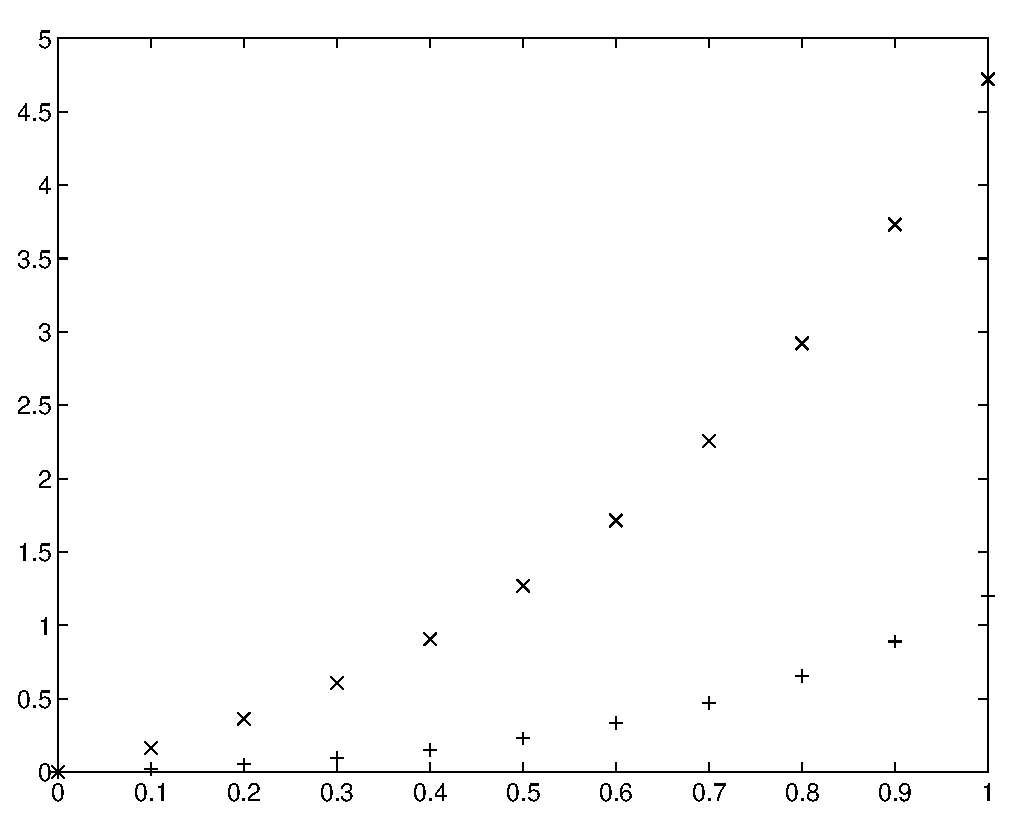
\psfig{file=figures/globerr3.eps,width=3.2in}}
   \caption{The global discretization error (marked by
   $+$) and its bound given in \protect\Ref{eq:geestimate}
   (marked by $\times$) for the step size $h=0.1$.}
   \label{fig:Lgeest}
\end{figure}

\subsection*{A Bound on Local Discretization Errors}
\index{error bound}

It remains to demonstrate how to determine a bound $\delta_h$ on
the local discretization error $\delta(k)$ for a given numerical 
method applied to the initial value problem
\begin{eqnarray*}
\frac{dx}{dt} & = & f(t,x)\\
x(t_0) & = & x_0,
\end{eqnarray*}
on the interval $[t_0,t_e]$.  Again we consider Euler's method.
The crucial tool for the computation of the local error is a Taylor
expansion of the solution combined with the fact that the 
derivatives of $x(t)$ can be written in terms of the function $f$
by the differential equation.  Using this idea we 
expand $x(t_{k+1})=x(t_k+h)$ up to second order by
\begin{eqnarray*}
x(t_{k+1})&=&
x(t_k)+h\frac{dx}{dt}(t_k)+\frac{h^2}{2}\frac{d^2x}{dt^2}(t_k+\theta h)\\
&=& x(t_k)+hf(t_k,x(t_k))+\frac{h^2}{2}\frac{d^2x}{dt^2}(t_k+\theta h),
\end{eqnarray*}
with an appropriate $0<\theta<1$.  Substitution into the expression
for the local error leads to
\begin{eqnarray*}
\delta(k+1)&=&x(t_{k+1}) - (x(t_k) + hf(t_k,x(t_k)))\\
&=& \frac{h^2}{2}\frac{d^2x}{dt^2}(t_k+\theta h).
\end{eqnarray*}
Hence, choosing a constant $C_E$ by
\[
C_E=\frac{1}{2}
\max\left\{ \left\vert\frac{d^2x}{dt^2}(s)\right\vert,\, t_0\le s\le t_e\right\},
\]
we find that $\delta(k+1)\le \delta_h$ for all $k$ if we set
\[
\delta_h = C_E h^2.
\]

Since the solution $x(t)$ of the initial value problem is in general
not known, it is more appropriate to find a bound for the
constant $C_E$ directly from the right hand side
$f$ in the differential equation.  We now outline a procedure
how this can be accomplished.

We have $\frac{dx}{dt}(t)=f(t,x(t))$ and it follows
\arraystart
\begin{equation}
\label{eq:Taylor2}
\begin{array}{rcl}
\dps\frac{d^2x}{dt^2}(t) &=& \dps\frac{\partial f}{\partial t}(t,x(t))
+\frac{\partial f}{\partial x}(t,x(t))\frac{dx}{dt}(t)\\
&=& \dps\frac{\partial f}{\partial t}(t,x(t))
+\frac{\partial f}{\partial x}(t,x(t))f(t,x(t)).
\end{array}
\end{equation}
\arrayfinish
Hence if a solution has to be computed for $t_0\le t\le t_e$, and the
values of the solution certainly are in the range $x_\ell \le x \le x_u$, then
\begin{equation} \label{eq:CE}
C_E\le \frac{1}{2}\max\left\{ \left\vert\frac{\partial f}{\partial t}(s,y)
+\frac{\partial f}{\partial x}(s,y)f(s,y)\right\vert,\, t_0\le s\le t_e,\quad
x_\ell \le y \le x_u \right\}.
\end{equation}

As an example of \Ref{eq:CE} we approximate the solution of the initial 
value problem
\begin{eqnarray*}
\frac{dx}{dt} & = & 5 x\\
 x(0) & = & 1,
\end{eqnarray*}
on the interval $[0,T]$.  Here $f(t,x)=5 x$ and therefore
\[
\frac{\partial f}{\partial t}(t,x)=0\AND
\frac{\partial f}{\partial x}(t,x)=5.
\]
From the ODE we see that the solution is monotonically increasing
and thus we find that
\[
C_E\le \frac{1}{2}\max\left\{ \left\vert 0+5\cdot 5y\right\vert,
y=x(T) \right\} = \frac{25}{2}x(T).
\]
Therefore we can choose
\[
\delta_h = \frac{25}{2}\bar x h^2
\]
for any $\bar x$ such that $\bar x \ge x(T)$.  In particular,
we have confirmed the result we have previously obtained, 
see \Ref{eq:dhlam}.

The computation of the local discretization error using Taylor expansions 
is quite tedious.  Therefore we just remark here that
for the modified Euler 
method\index{modified Euler method!local discretization error} 
the local error can be bounded by a function
of the form
\[
\delta_h = C_Mh^3,
\]
and for the fourth order Runge-Kutta 
method\index{fourth order Runge-Kutta method!local discretization error} 
\index{Runge-Kutta method!fourth order!local discretization error} 
the local discretization error is bounded by
\[
\delta_h = C_R h^5.
\]
Here $C_M$ and $C_R$ are positive constants.  

\subsection*{A Bound on Global Discretization Errors}

Once the local discretization error is bounded we can use
Theorem~\ref{prop:glerr} to obtain a bound on global discretization 
error.  In particular, we can prove:
\begin{prop} \label{prop:errEMR}
Suppose that \Ref{eq:PhiLip} holds.  Then there are constants $C_E$,
$C_M$ and $C_R$ such that the global discretization error of
\begin{itemize}
\item[(a)] \index{Euler's method!global discretization error}
Euler's method is bounded by
\[
|\epsilon(k)| \le \frac{e^{khL}-1}{L}C_E h;
\]
\item[(b)] \index{modified Euler method!global discretization error}
the modified Euler method is bounded by
\[
|\epsilon(k)| \le \frac{e^{khL}-1}{L}C_M h^2;
\]
\item[(c)] \index{fourth order Runge-Kutta method!global discretization error}
\index{Runge-Kutta method!fourth order!global discretization error} 
the fourth order Runge-Kutta method is bounded by
\[
|\epsilon(k)| \le \frac{e^{khL}-1}{L}C_R h^4.
\]
\end{itemize}
\end{prop}

In view of this proposition it is clear that the fourth order Runge-Kutta 
method is much better than Euler's method or the modified
Euler method: the reason is that for small step sizes $h$ the value of 
$h^4$ is much smaller than $h^2$ or even $h$ itself.  Hence the
global discretization error of the fourth order Runge-Kutta method is,
for reasonably small step sizes, much smaller than for the other two
methods.  In addition, it is also evident how the {\em fourth order\/} 
Runge-Kutta method got its name.

\subsubsection*{Specifying the Tolerance}

In principle, we can use Proposition~\ref{prop:errEMR} to find a step 
size for which the global discretization error is not bigger than a
specified tolerance.  To illustrate this point,  
consider the initial value problem (see also \Ref{eq:eulexivp})
\begin{eqnarray*}
\frac{dx}{dt} & = & x+t \\
x(1) & = & 2.
\end{eqnarray*}
The aim is to find a step size $h$ such that Euler's method is
approximating the solution on the interval $[1,3]$ up to a global 
discretization error smaller than $0.1$.  By Proposition~\ref{prop:errEMR}
this can be guaranteed if $h$ is chosen so that
\[
\frac{e^{khL}-1}{L}C_E h < 0.1.
\]
For this example $L=1$, since
\[
|y+t-(z+t)|=|y-z|=1\cdot |y-z|.
\]

We now find a bound for the constant $C_E$.  We compute
\[
\frac{\partial f}{\partial t}(s,y)=\frac{\partial f}{\partial x}(s,y)=1.
\]
We see from the ODE that the solution is monotonically increasing.
Suppose that we know that for $t\in [1,3]$ the solution $x(t)$ is bounded
by $40$ from above.  Using \Ref{eq:CE} we obtain an estimate for $C_E$ by
\[
C_E\le \frac{1}{2}\max\left\{\vert 1+1\cdot f(s,y)\vert,\, 1\le s\le 3,\,
2 \le y \le 40 \right\}=\frac{44}{2}=22.
\]
Since $e^{kh}\le e^{t_e-t_0}=e^2$, we can choose an $h$ such that
\[
(e^2-1)22h < 0.1\quad \Longleftrightarrow 
\quad h<\frac{1}{220(e^2-1)}\approx 0.00071.
\]
Indeed, computing a solution with \Matlab by
\begin{verbatim}
h     = 0.0007;
t(1)  = 1;
x(1)  = 2;
K     = round(2/h);
for k = 1:K
     t(k+1) = t(k)+h;
     x(k+1) = x(k)+h*(x(k)+t(k));
end
plot(t,x)
xlabel('t')
ylabel('x')
\end{verbatim}
we obtain the result in Figure~\ref{fig:hsmall}.  (The \Matlab
command {\tt round} rounds a number towards the nearest integer.)
The outcome cannot be distinguished from the exact solution shown 
in Figure~\ref{fig:eulex1}(b).

\begin{figure}[htb]
   \centerline{%
   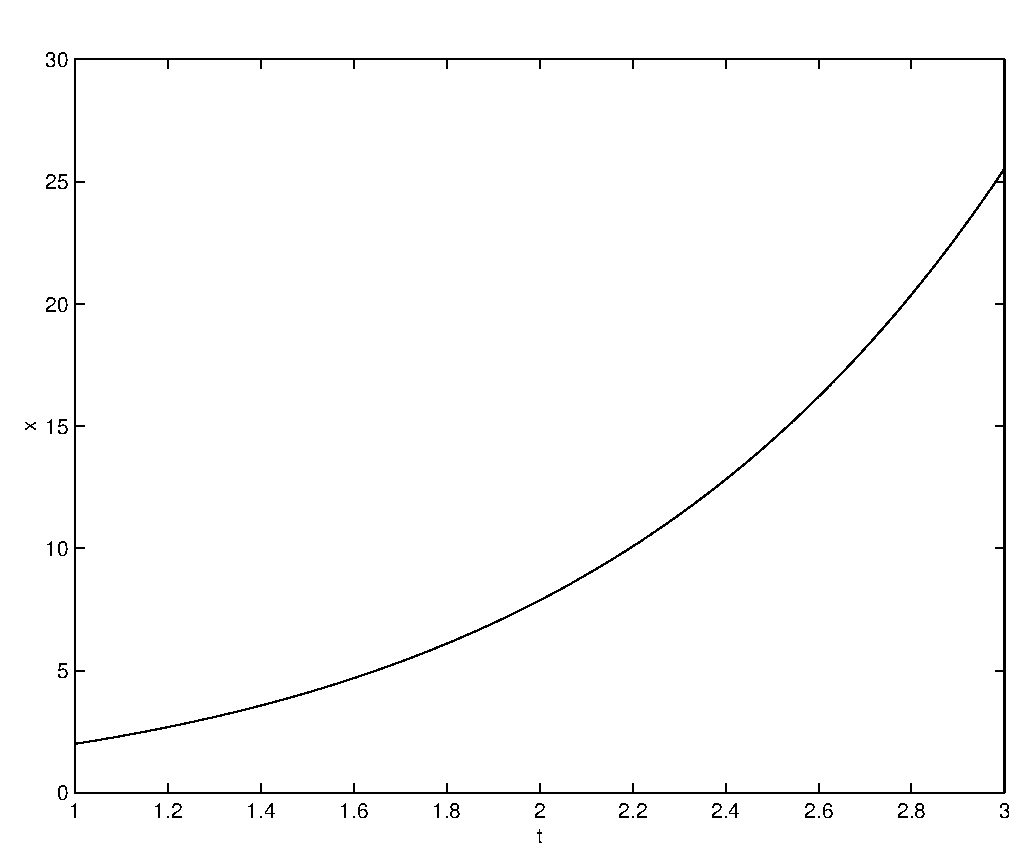
\psfig{file=figures/globerr6.eps,width=3.2in}}
   \caption{The numerical solution obtained by Euler's method for the 
   step size $h=0.0007$.}
   \label{fig:hsmall}
\end{figure}

\EXER

\TEXER

\begin{exercise} \label{c15.3.1}
Determine the function $\Phi=\Phi(t_k,x_k,h)$ which belongs to the 
fourth order Runge-Kutta method.
\end{exercise}

\noindent In Exercises~\ref{c15.3.2a} -- \ref{c15.3.2b} find an estimate
for the constant $C_E$ of the form $C_E \le Kx(t_0)$ where $x(t)$ is the
solution of the specified initial value problem on $[0,T]$ and $t_0\in[0,T]$.
\begin{exercise} \label{c15.3.2a}
$\dps\frac{dx}{dt} = 3 x$ where $x(0) = 2$.
\end{exercise}
\begin{exercise} \label{c15.3.2b}
$\dps\frac{dx}{dt} = -x$ where $x(0) = 1$.
\end{exercise}


\CEXER

\begin{exercise} \label{c15.3.3}
Set $\lambda=0.2$ and the step size $h=0.1$.  Use \Matlab to compute 
the global discretization error and its bound in \Ref{eq:geestimate}
on the interval $[0,1]$.  Compare the result with the ones obtained 
in Figures~\ref{fig:globerr1} and \ref{fig:Lgeest}.
\end{exercise}



\end{document}
